\documentclass{standalone}
\usepackage{tikz}
\usetikzlibrary{positioning, arrows.meta}

\begin{document}
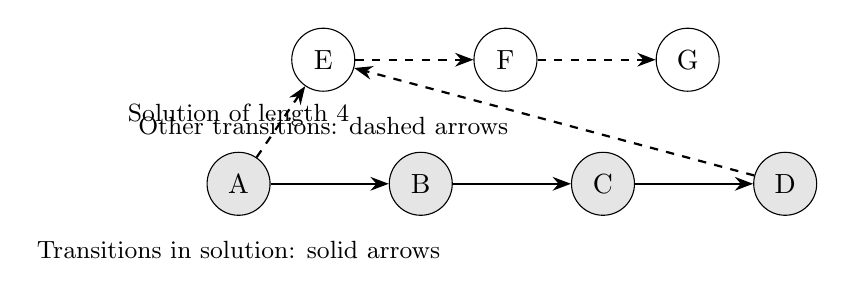
\begin{tikzpicture}[
    node distance=1.5cm,
    solution_node/.style={circle, draw, fill=gray!20, minimum size=0.8cm},
    normal_node/.style={circle, draw, minimum size=0.8cm},
    arrow/.style={-Stealth, thick},
    dashed_arrow/.style={-Stealth, thick, dashed}
]

% Solution nodes (gray background)
\node[solution_node] (A) at (0, 0) {A};
\node[solution_node] (B) [right=of A] {B};
\node[solution_node] (C) [right=of B] {C};
\node[solution_node] (D) [right=of C] {D};

% Non-solution nodes
\node[normal_node] (E) [above right=1cm and 0.5cm of A] {E};
\node[normal_node] (F) [right=of E] {F};
\node[normal_node] (G) [right=of F] {G};

% Solution transitions (solid arrows)
\draw[arrow] (A) -- (B);
\draw[arrow] (B) -- (C);
\draw[arrow] (C) -- (D);

% Non-solution transitions (dashed arrows)
\draw[dashed_arrow] (A) -- (E);
\draw[dashed_arrow] (E) -- (F);
\draw[dashed_arrow] (F) -- (G);
\draw[dashed_arrow] (D) -- (E);

% Optional: Add labels for clarity
\node[above=0.2cm of A] {\small Solution of length 4};
\node[below=0.2cm of A] {\small Transitions in solution: solid arrows};
\node[below=0.2cm of E] {\small Other transitions: dashed arrows};

\end{tikzpicture}
\end{document}